%TEX root = ../dokumentation.tex

\chapter{Datencrawler}

\section{Vorüberlegung}
Der zu entwickelnde Datencrawler soll mit Hilfe einer IBM Connections Seedlist-\ac{URL} die vollständige Seedlist herunterladen und im JSON-Format an eine API senden. Dazu muss das Programm sich zunächst authentifizieren, dann den Inhalt herunterladen und sortieren und weitergeben. Danach wird nach einer Folge-\ac{URL} gesucht und dementsprechend entweder die nächste Seite der Seedlist bearbeitet oder der Timestamp abgespeichert. Zu bedenken sind dabei die Fehlerszenarien, die eintreten können. Die Authentifizierung spielt dabei eine Rolle, ebenso mögliche Fehler bei der Durchführung von einzelnen Schritten.
\begin{figure}[ht]
\centering
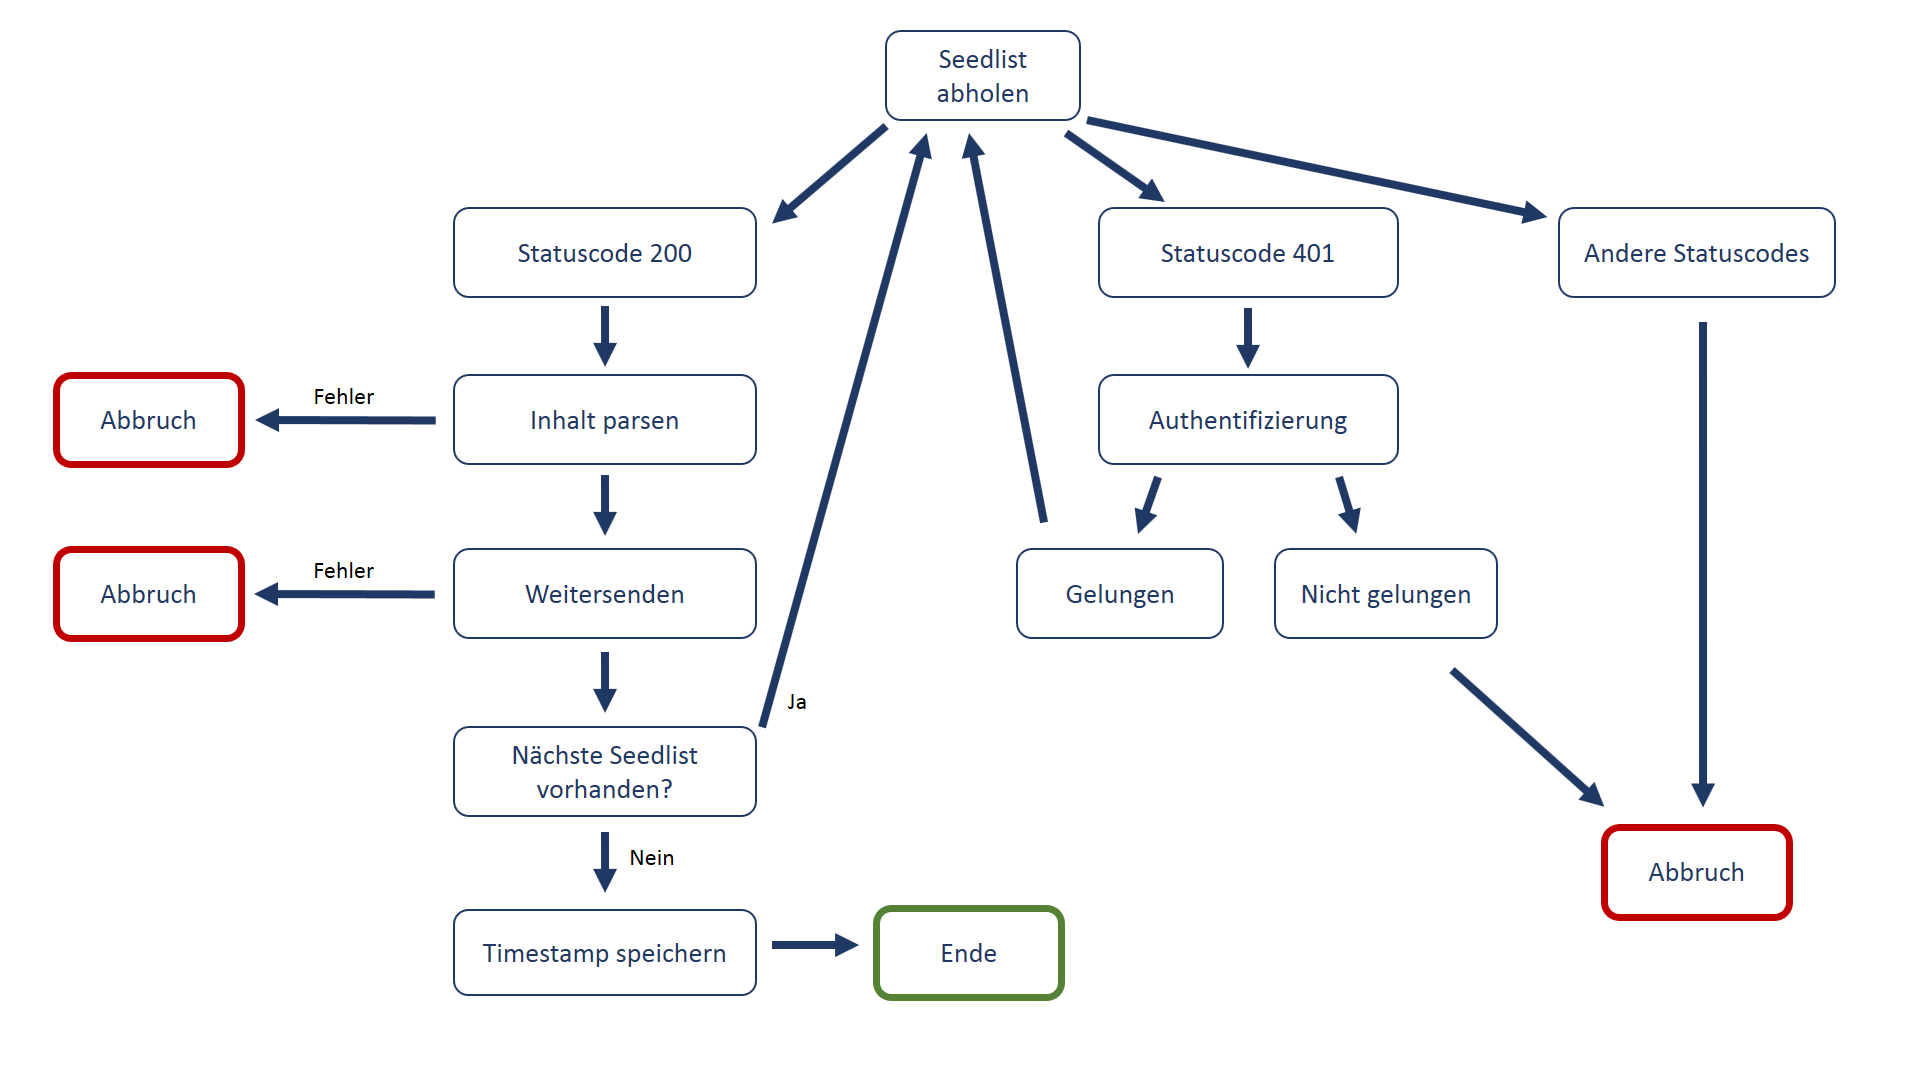
\includegraphics[width=1.0\textwidth, height=10cm]{Ablauf.png}
\caption{Ablauf des Programms}
\end{figure}

Im ersten Schritt soll der Crawler einmal versuchen, eine Seedlist abzuholen. Wenn dies nicht erfolgreich war und der HTTP-Statuscode \textit{401 Unauthorized} ist, bedeutet dies, dass das Token für die Authentifizierung abgelaufen ist oder noch keines angefordert wurde. Daher muss das Programm einen neuen Token bekommen und versucht, sich zu authentifizieren. Gelingt dies nicht, bricht es ab. Würde es erneut versuchen, sich zu authentifizieren und dies erneut fehlschlagen, würde dieser Ablauf immer wieder wiederholt werden und so eine unendliche Schleife bilden. Bei Erfolg versucht es erneut, sich die Seedlist zu holen. Sollte die Antwort bei dem Abruf der Seedlist ein anderer Statuscode als \textit{200 OK} oder \textit{401 Unauthorized} sein, hat das Programm keine weitere Möglichkeit, auf die Seedlist zuzugreifen und bricht ab.

Gelingt der Abruf, kann der Inhalt der Seedlist verarbeitet werden. Da dieser in Form von XML bereitgestellt wird, muss er zunächst geparsed werden. Danach werden die für den Expertise Locator relevanten Daten gefiltert und in ein JSON-Objekt überführt. Wenn in diesem Vorgang ein Fehler auftritt, wird das Programm abgebrochen.

Der nächste Schritt ist das übergeben der Informationen an eine \acs{API}, die diese entsprechend in eine Datenbank einsortiert. Damit ist eine Seite einer Seedlist verarbeitet. Nun wird überprüft, ob es eine Folge-\ac{URL} gibt. Ist dies der Fall, beginnt der soeben beschriebene Prozess mit der entsprechenden Folge-URL von vorn. Gibt es keine Folge-\ac{URL}, existiert stattdessen ein Timestamp, der abgespeichert wird, um zukünftig beim Crawlen nicht mehr alle Informationen von der Seedlist zu bekommen, sondern nur noch die Änderungen seit diesem Timestamp.

\newpage


\section{Lösung}
